%%%%%%%%%%%%%%%%%%%%%%%%%%%%%%%%%%%%%%%%%
% fphw Assignment
% LaTeX Template
% Version 1.0 (27/04/2019)
%
% This template originates from:
% https://www.LaTeXTemplates.com
%
% Authors:
% Class by Felipe Portales-Oliva (f.portales.oliva@gmail.com) with template 
% content and modifications by Vel (vel@LaTeXTemplates.com)
%
% Template (this file) License:
% CC BY-NC-SA 3.0 (http://creativecommons.org/licenses/by-nc-sa/3.0/)
%
%%%%%%%%%%%%%%%%%%%%%%%%%%%%%%%%%%%%%%%%%

%----------------------------------------------------------------------------------------
%	PACKAGES AND OTHER DOCUMENT CONFIGURATIONS
%----------------------------------------------------------------------------------------

\documentclass[
  french,
  % twocolumn,
	11pt, % Default font size, values between 10pt-12pt are allowed
	%letterpaper, % Uncomment for US letter paper size
	%spanish, % Uncomment for Spanish
]{fphw}

% \usepackage[fontsize=10.0]{scrextend} % Use this to force the fontsize

%% Commands for numbering paragraphs
\renewcommand\thesection{\Roman{section}}
\renewcommand\thesubsection{\thesection.\arabic{subsection}}
\renewcommand*\thesubsubsection{%
  \Roman{section}.\arabic{subsection}.\alph{subsubsection}%
}

\usepackage{sectsty}
\sectionfont{\bfseries\Large\raggedright}

% Template-specific packages
\usepackage{babel}
\usepackage[utf8]{inputenc} % Required for inputting international characters
% \usepackage{DejaVuSerifCondensed} 
\usepackage[T1]{fontenc} % Output font encoding for international characters

\usepackage{kpfonts}        %% For math only
\usepackage{fontspec}       %% Because we are using XeTEX
\setromanfont{Minion Pro}   %% For text (Minion Math is commercial)

%-----------------------------------------------------------------------
% \setromanfont{Meta Serif Pro}
% \setsansfont{Fira Sans}
% \setmonofont[Color={0019D4}]{Fira Code} 
%-----------------------------------------------------------------------

\usepackage{fancyvrb}
\usepackage{fvextra}
\newcommand\userinput[1]{\textbf{#1}}
\newcommand\arguments[1]{\textit{#1}}

\usepackage{amsmath}
\usepackage{mathtools}
\usepackage{xfrac} 

\usepackage{graphicx} % Required for including images
\usepackage[textfont=it,font=small]{caption}  %% To manage long captions in images
\usepackage{subcaption}
\captionsetup{justification=centering}

\usepackage{float}
\graphicspath{ {../img/} }

\usepackage{booktabs} % Required for better horizontal rules in tables

\usepackage{listings} % Required for insertion of code

\usepackage{array} % Required for spacing in tabular environment

\usepackage{enumerate} % To modify the enumerate environment

\usepackage{amssymb}
\usepackage{enumitem}	%% % To modify the itemize bullet character

\newcommand{\tabhead}[1]{{\bfseries#1}}

\usepackage{xcolor}
\usepackage{listings}
\colorlet{mygray}{black!30}
\colorlet{mygreen}{green!60!blue}
\colorlet{mymauve}{red!60!blue}
\lstset{
  backgroundcolor=\color{gray!10},  
  basicstyle=\ttfamily,
  columns=fullflexible,
  breakatwhitespace=false,      
  breaklines=true,                
  captionpos=b,                    
  commentstyle=\color{mygreen}, 
  extendedchars=true,              
  frame=single,                   
  keepspaces=true,             
  keywordstyle=\color{blue},      
  language=c++,                 
  numbers=none,                
  numbersep=5pt,                   
  numberstyle=\tiny\color{blue}, 
  rulecolor=\color{mygray},        
  showspaces=false,               
  showtabs=false,                 
  stepnumber=5,                  
  stringstyle=\color{mymauve},    
  tabsize=3,                      
  title=\lstname                
}

\usepackage[linkcolor=blue,colorlinks=true]{hyperref}
% \usepackage[colorlinks=true,urlcolor=blue]{hyperref}
\hypersetup{citecolor=blue}

\usepackage{cleveref}
\usepackage{siunitx}
\usepackage{bm}

\usepackage[backend=bibtex,style=alphabetic,maxnames=2,natbib=true]{biblatex} % Use the bibtex backend with the alphabetic citation style (compact APA-like)
% \usepackage[backend=bibtex,style=authoryear,maxnames=2,natbib=true]{biblatex} % Use the bibtex backend with the authoryear citation style (which resembles APA)
\addbibresource{../bib/bibliography.bib} % The filename of the bibliography
\usepackage[autostyle=true]{csquotes} % Required to generate language-dependent quotes in the bibliography 
% \renewcommand*{\bibfont}{\tiny} % Pour reduire la taille des references

\usepackage[useregional=numeric]{datetime2}
\usepackage[normalem]{ulem}

% %-------------------------------------------------------------------------------

\newcommand{\myvec}[3]{\begin{pmatrix} #1  \\ #2 \\ #3 \end{pmatrix}}   %% vecteur 3d
\newcommand{\mymat}[9]{\begin{pmatrix} #1 & #2 & #3 \\ #4 & #5 & #6 \\ #7 & #8 &#9 \end{pmatrix}}  %% Matrice 3*3

\renewcommand{\vector}[4]{\begin{pmatrix} #1  \\ #2 \\ #3 \\ #4 \end{pmatrix}}   %% vecteur 4d
% \newcommand{\mymatrix}[16]{\begin{pmatrix} #1 & #2 & #3 & #4 \\ #4 & #6 & #7 & #8 \\ #9 & #10 & #11 & #12 \\ #13 & #14 & #15 & #16 \end{pmatrix}}  %% Matrice 3*3

\newcommand{\hquad}{\hspace{0.5em}} %% Bew command for half quad
\newcommand*\diff{\mathop{}\!\mathrm{d}}
% \setlength\parindent{0pt}	%% To remove all indentations
\newcommand{\bvec}[1]{\bm{\mathrm{#1}}}  %% Use this to make vectors
\newcommand{\bmat}[1]{\bm{\mathsf{#1}}}   %% Use this to make tensors

%----------------------------------------------------------------------------------------
%	ASSIGNMENT INFORMATION
%----------------------------------------------------------------------------------------

\title{Compte rendu semaine \#9} % Assignment title
% \title{Difficultés rencontrées} % Assignment title

\author{Roussel Desmond Nzoyem} % Student name

\date{\DTMdisplaydate{2021}{3}{31}{-1} - \DTMdisplaydate{2021}{4}{06}{-1}} % Due date

\institute{Sorbonne Université \\ Laboratoire Jacques-Louis Lions} % Institute or school name

\class{Stage M2} % Course or class name

\professor{Pr. Stéphane Labbé} % Professor or teacher in charge of the assignment

%----------------------------------------------------------------------------------------

\begin{document}

\maketitle % Output the assignment title, created automatically using the information in the custom commands above

%----------------------------------------------------------------------------------------
%	ASSIGNMENT CONTENT - INTRO
%----------------------------------------------------------------------------------------


Cette semaine a été consacrée à l'étude du modèle de percussion 1D. J'ai developé un modèle de collision complètement inélastique (les deux floes deviennemt un seul objet à la fin du choc). Ce modèle permettra à terme (après résolution graduelle des nombreuses simplifications qui ont été faites) d'introduire la percussion 1D.




%----------------------------------------------------------------------------------------
%	ASSIGNMENT CONTENT - SECTION 1
%----------------------------------------------------------------------------------------

\section*{Tâches effectuées}

\begin{enumerate}
  \item Lecture de plusieurs modèles de systèmes masses-ressorts avec dispositifs visqueux. Le document qui s'est montré le plus utile est \parencite{homodeling} grace à ses nombreux exemples illustrés.
  \item Ensuite il a fallu poser le porblème de percission 1D, et d'écrire les équations régissant le système (voir \textit{rapport de stage}).
  \item La troisième tâche à été de simuler le modèle à l'aide des librairies \verb|scipy| et \verb|bokeh|. Cette simulation interactive a permis de constater des erreurs dans le modèle qui ont aussitot corrigées (voir \textit{notebook} rataché). 
\end{enumerate}


%----------------------------------------------------------------------------------------
%	ASSIGNMENT CONTENT - SECTION 2
%----------------------------------------------------------------------------------------

\section*{Difficultés rencontrées}

\textit{Le rapport de stage et un notebook Python sont rataché à ce rapport.}

\begin{enumerate}
  \item La permière question concerne la condition initiale sur le modèle 1D qui a été crée: \textit{la vitesse initiale de la masse $m+m'$ (dont le déplacement est noté $x_1$) est-elle vraiment nulle ?} \textbf{En fait non, cette vitesse ne peut être nulle !} je compte isoler le système (en supprimant le mur à gauche) afin d'utiliser la \textbf{conservation de la quantité de mouvements} ; ceci pour déduire la vitesse "initiale" de l'ensemble $m+m'$ après collision et fixation de $m'$ (de vitesse $-v_0$) sur $m$ (de vitesse nulle).
  \begin{figure}[H]
    \centering
    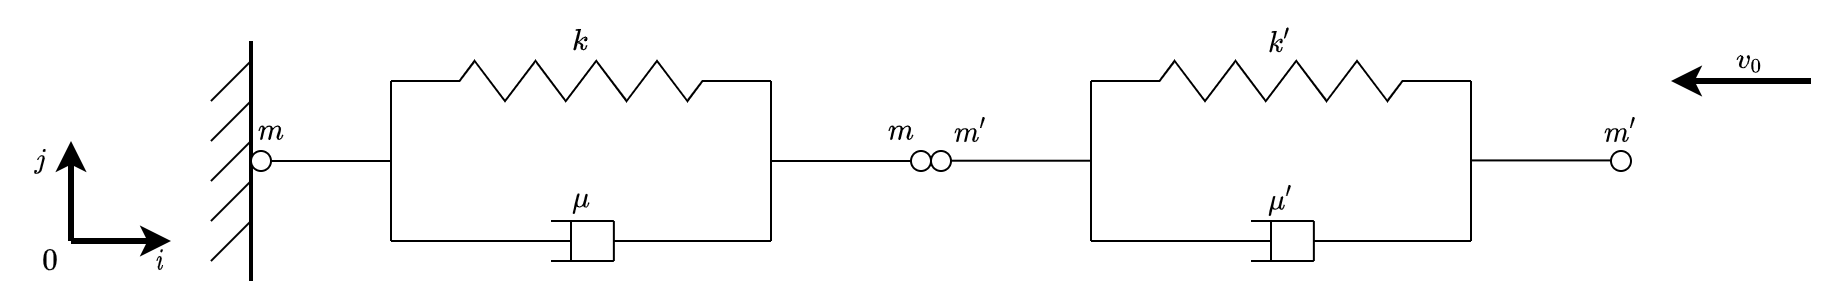
\includegraphics[width=0.8\textwidth]{Percussion1D-Systeme.png}
    \caption{Modèle de collision 1D entre deux floes modélisés par des réseaux de ressorts à deux noeuds chacuns; à l'instant initial, le premier est imobile, et le deuxième se déplace à la vitesse $-v_0$.}
  \end{figure}
  \item La deuxième question est la même que celle de la semaine dernière (question 2): \textit{dans la résolution du problème lineaire de complementarité régissant la collision, les forces de contact dépendent des position des noeuds durant la très brève percussion}. Pour résoudre ce problème en 1D (et calculler les vitesses après contact inélastique\footnote{Le conctat cette fois sera tout juste inélastique, il ne sera plus parfaitement inélastique; i.e. les deux floes se séparent après contact.}), je compte utiliser le modèle décrit ci-haut (à la question 1) durant le phase de \textbf{dynamique non-régulière} pour déterminer les positions et les vitesses des différents noeuds. Celà permettra de calculer les forces exercées sur les noeuds \textbf{en tout temps}.
\end{enumerate}

%----------------------------------------------------------------------------------------
%	ASSIGNMENT CONTENT - SECTION 3
% ----------------------------------------------------------------------------------------

\section*{Travail à venir}

\textit{En supposant que je suis sur la bonne voie, je me consacrerais aux tâches suivantes durant les semaines à venir (par ordre de priorité).}
\begin{enumerate}
  \item Isolation du système 1D et calcul de la vitesses "initiale" de la masse $m+m'$.
  \item Toujours en 1D, calcul analytique et numérique des état d'équilibres du système d'EDO (collision parfaitement inélastique); distinguer les états stables des autres.
  \item Calculer analytiquement la solution du système d'EDO; déduire la condition sur les paramètres pour que le système converge vers l'état d'équilibre voulu.
  \item Intégration du modèle dans un problème linéaire de complémentarité en 1D. On obtiendra ainsi les vitesses de chacun des blocs détachés après contact.
  \item Passage au modèle 2D.
  \item Passage à l'étude de la fracture après percussion.
\end{enumerate}



% %-------------------------------------------------------------------------------
% %							THE BIBLIOGRAPHY
% %-------------------------------------------------------------------------------
\clearpage   % Pour retirer les references de la bare de navigation
\printbibliography


\end{document}
